\section{Experimental Evaluation}
\label{sec:exp}

% exp goals 
%\tian{Important to change}
%Our evaluation focus on answering the following questions: 
%(1)	First, we study the lifetime of transient GPU servers and make an observation about the revocation pattern. This revocation pattern is then be used to perform simulation. 
%(2)	What is the most suitable communication architecture of distributed training, considering the revocation pattern? For this, we experiment with both synchronous and asynchronous, as well as allreduce architectures. 
%(3)	What is the performance impact of training with heterogeneous GPU servers in the same training session? The motivation to investigate this question is because the inherent needs to use whatever transient servers are available to improve the training speed.
%(4)	What are the network characteristics of parameter-server based distributed training? And what is the relationship between model size, network bandwidth, and network latency?   
%(5)	What is the performance impact of training with servers from geographically distributed cloud locations? 


%Our evaluation focus on answering the following key research questions through empirical measurement studies:
%\begin{itemize}
%\item What are the training performance when using transient servers? 
%\item What are the potentials of dynamic transient training compared and challenges associated with it? 
%\item What are the performance impact on distributed transient training with heterogeneous server resources both in terms of server type and locations? 
%\end{itemize}

Our evaluation focuses on answering the following key research questions:
(1) How do transient servers compare to on-demand servers with respect to distributed training? 
(2) What is the best cluster configuration given a fixed monetary budget?
(3) How does revocation of transient servers impact distributed training? 
(4) What are the potential benefits and challenges associated with dynamic clusters? 
(5) What is the performance impact when using heterogeneous server resources? 
%In investigating the distributed training performance with transient servers, we uncover the inefficiency of current cloud revocation policies and distributed training frameworks. 


%In the following sections, we first describe the experiment setups, followed by empr
%Our study reveals.... and motivates the redesign of distributed deep learning frameworks.... 

%Last, we describe our key research questions and
%summarize the empirical measurements  that shed light on future redesigns of 
%distributed deep learning frameworks. 

\begin{table}[t!]
\centering
\resizebox{0.48\textwidth}{!}{%
\begin{tabular}{@{}ccccccc@{}}
\toprule
\textbf{\begin{tabular}[c]{@{}c@{}}GCE \\ instance\end{tabular}} & \textbf{\begin{tabular}[c]{@{}c@{}}Mem.\\ (GB)\end{tabular}} & \textbf{vCPU} & \textbf{\begin{tabular}[c]{@{}c@{}}On-demand\\ (\$/hr)\end{tabular}} & \textbf{\begin{tabular}[c]{@{}c@{}}Transient\\ (\$/hr)\end{tabular}} & \textbf{\begin{tabular}[c]{@{}c@{}}Saving \\ potential(\%)\end{tabular}} & \textbf{\begin{tabular}[c]{@{}c@{}}EC2\\ counterpart\end{tabular}} \\ \midrule
\textit{K80} & 61 & 4 & 0.723 & 0.256 & 35.4 & p2.xlarge \\
\textit{P100} & 61 & 8 & 1.43 & 0.551 & 38.5 & - \\
\textit{V100} & 61 & 8 & 2.144 & 0.861 & 40.2 & p3.2xlarge \\
\rowcolor[HTML]{EFEFEF} 
\textit{PS} & 16 & 4 & 0.143 & 0.041 & - & m4.xlarge \\ \midrule
\textbf{\begin{tabular}[c]{@{}c@{}}CNN \\ model\end{tabular}} & \textbf{\begin{tabular}[c]{@{}c@{}}Num. \\ parameters\end{tabular}} & \textbf{\begin{tabular}[c]{@{}c@{}}Model size \\ (MB)\end{tabular}} & \textbf{\begin{tabular}[c]{@{}c@{}}Num. \\ layers\end{tabular}} & \textbf{\begin{tabular}[c]{@{}c@{}}Batch \\ size\end{tabular}} & \textbf{\begin{tabular}[c]{@{}c@{}}Top-1 \\ accuracy(\%)\end{tabular}} & \textbf{Optimizer} \\
\textit{ResNet-32} & 1.9M & 14.19 & 32 & 128 & 92.49 & Momentum \\ \bottomrule
\end{tabular}%
}
\caption{\textbf{Server configurations and models used in our
  experiments.} We customized both GPU servers (used to run workers) and a CPU
  server (shaded and referred to as \textit{PS}) in Google Cloud Engine. The
  first column specifies the type of GPU cards used for each server. 
  %We
  %choose the amount of memory and vCPU based on Amazon EC2 counterparts, with
  %the goal to enable fair comparisons across cloud platforms in future works.
  %We run parameter server using on-demand server to simplify the failure
  %%recovery and also the on-demand price of PS is only about half of the
  %cheapest GPU transient server \texttt{K80}. 
  For \emph{ResNet-32}, the top-1
  accuracy is obtained from the original paper that evaluates against Cifar-10
  dataset.}
%   \tian{For end-to-end evaluation (trained to converging), unless
%  otherwise specified, ResNet-32 is used. All other models are used to
%  understand the model size impact on distributed training speed.}}
\label{tbl:exp_setup}
\end{table}

\subsection{Experimental Setup}
\label{subsec:setup}

\paragraph{Public Cloud Infrastructure} 

We conducted our experiments using Google Compute Engine (GCE) and the server
configurations shown in Table~\ref{tbl:exp_setup}. We choose three GPU server
configurations with different GPU capacities---\texttt{K80}, \texttt{P100}, and
\texttt{V100} in increasing order of GPU memory, parallel cores, etc.   For simplicity of
exposition, we refer to each GPU server configuration by the attached  GPU.

To better avoid memory and CPU bottlenecks in our evaluation, we choose the max
memory and virtual CPU values allowed by GCE for each
configuration. 

The \emph{saving potential} illustrates the cost difference between 
\emph{transient} and \emph{on-demand} instances. It is calculated as the unit on-demand price divided
by the unit transient cost. 

The fourth server in Table~\ref{tbl:exp_setup}, labeled \texttt{PS}, was used
to run the parameter server during distributed training. This server did not
have an attached GPU---hence, the reduced cost---and was also run using an
on-demand instance.  The reason we use an on-demand instance for the parameter
server for distributed training is to circumvent the checkpoint restarts that would result if
parameter server is revoked. % note that, PS failed only lead to session failure, and once detected, then we have to restart from the last checkpoint model
%when training is to avoid the checkpoint restarts that would result if
%parameter server is revoked. 
However, we do use transient parameter servers
when measuring the lifetime of transient CPU server. 

\paragraph{Deep Learning Framework} 

We leveraged the popular deep learning framework TensorFlow~\cite{tensorflow} for all our
experiments given the relative maturity of the project and support for distributed training. 
We also used the Tensor2tensor library~\cite{tensor2tensor} to assist in the training process. 

For the model, we selected  \emph{RestNet-32}~\cite{resnet}, in part, due to its popularity. This 
CNN model can be trained to convergence using a single GPU server in $\sim$4
hours, making it practical for our experiments.  See Table~\ref{tbl:exp_setup}
for full model details.  

For the training dataset, we used, \emph{Cifar-10}~\cite{krizhevsky2009learning}, a standard image
recognition dataset consisting of 60K color images, each 32 by 32 pixels,
spanning 10 output classes. Following standard conventions in the field of deep
learning, we used 50K images for training and the rest for testing. We also
used the same hyperparameter configurations (e.g., learning rate) as specified
in the original paper for most of our experiments---any differences are noted
when appropriate.

\paragraph{Performance Metrics}

We focus on performance metrics that are most  relevant  to comparing
distributed training on transient servers to training on on-demand servers.
For transient servers, we monitor the revocation events and record their 
lifetimes respectively. For transient servers that were revoked by
GCE, their recorded lifetime will typically be shorter than the total training
time for the cluster.  Finally, a training cluster is said to have
\emph{failed} if the master worker is revoked prior to training completion.

For distributed training, we measure training time, training cost, and
accuracy.  Training time is defined as the amount of time required to complete
the specified training workload. When training the \emph{RestNet-32} model, we
specify the training workload to be \emph{64K} steps where each step equates to
processing a batch of 128 images in the \emph{Cifar-10} dataset. We refer to the model 
generated at  \emph{64K} steps as a \emph{converged model}.
 
Training cost is calculated using the sum of all cloud servers that participate
in the training process. In the case of distributed training, these include GPU
servers that are responsible of calculating the gradients and the CPU server
that is in charge of updating the model parameters. We calculate the cost of
each server by multiplying the unit cost by the amount of time that server was
active in training. For a transient server, the active training time stops when
the server is revoked or the training has completed. When analyzing the
training cost, we use a fine-grained second-based charging model~\cite{billing}. For
example, if the active training time is 3601 seconds, we will charge the server
for 3601 seconds. In the traditional hour-based charging model, the cost would
instead be based on two hours. Regardless of the charging model, we can
amortize the cost effectively when  transient training is offered as a service
in which different training sessions can share the training servers. 

Training accuracy is measured as the top-1 accuracy, i.e., the percentage of
correctly predicted images using the trained model on the test portion of the
dataset. In the case of the \emph{RestNet-32} model, we evaluate accuracy after
\emph{64K} steps. While our goal is not to increase the accuracy of existing models,
it is important to demonstrate that distributed training with transient servers
does not have a significant negative impact on accuracy. 





%%%%%

\subsection{Transient vs. On-demand Servers}
\label{subsec:trans_v_ondemand}


\begin{figure}[t]
\centering
    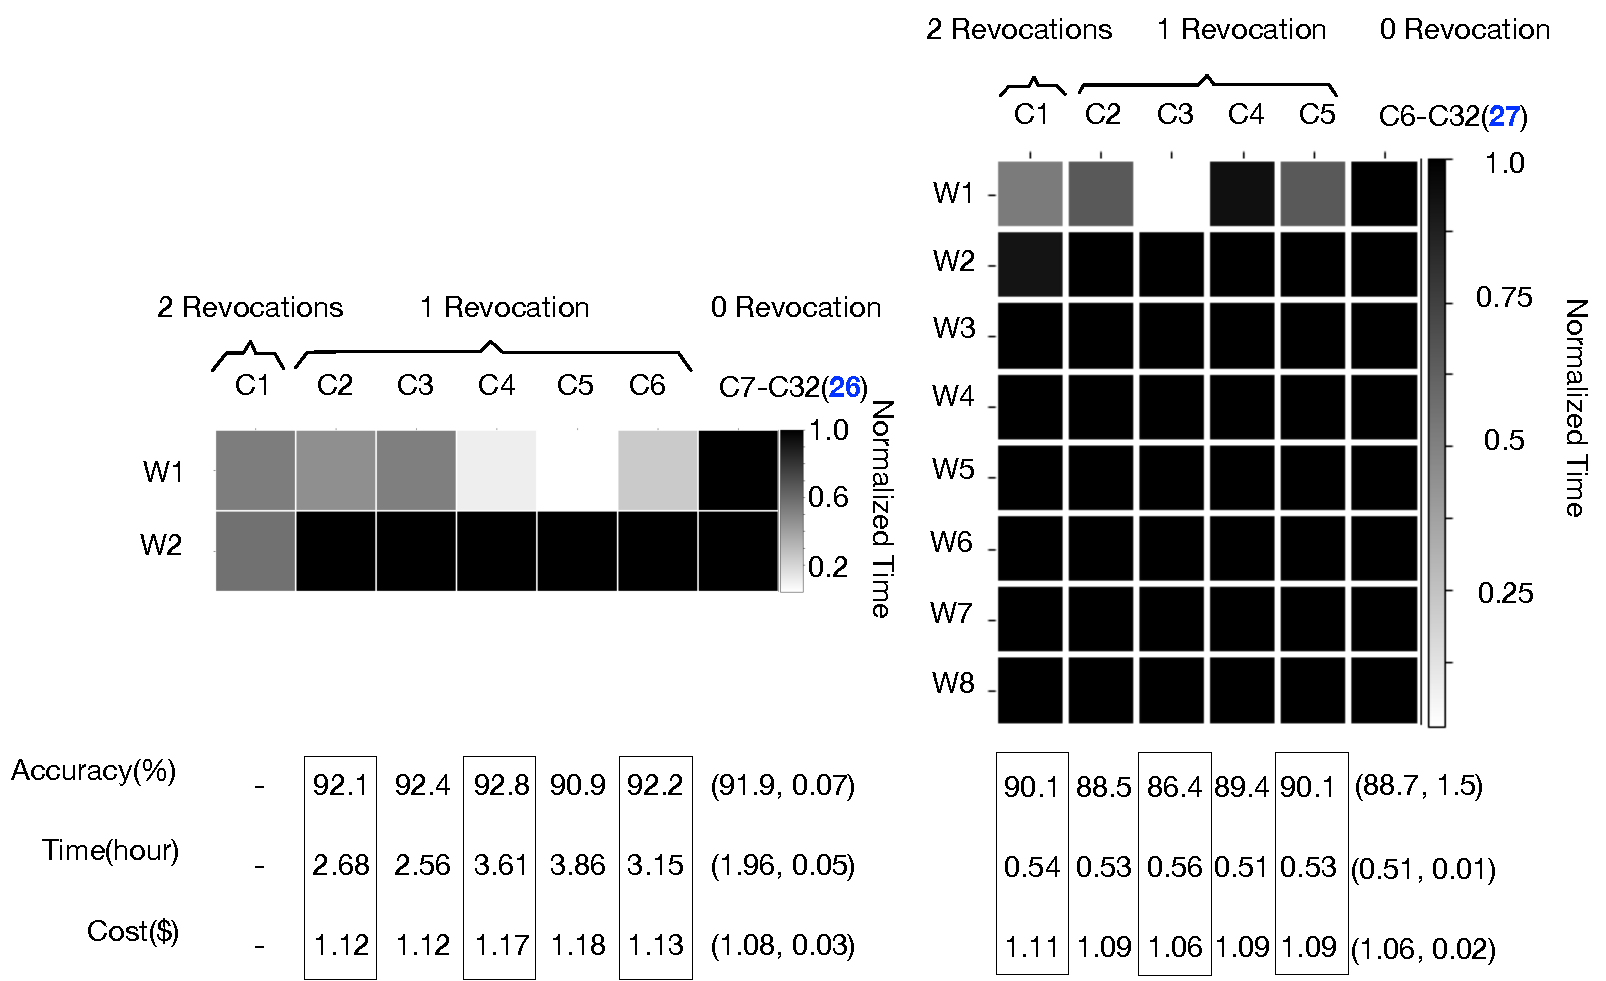
\includegraphics[width= \columnwidth ]{cluster_2_8_spots_heatmap.pdf}
\caption{\textbf{Performance comparison between distributed training using transient and on-demand GPU servers.} 
We measure the distributed training performance with three different cluster sizes. We repeat each cluster size 32 times and label them as $C_i$ where $i \in [1, 32]$. 
The cluster runs are sorted by the number of revocations and the workers $W_j$ are sorted by their lifetime. 
On average, using transient servers can achieve up to 62.9\% cost savings and up to 7.7X training speed up when compared to training using one \texttt{K80} on-demand server. 
%The training time and cost variations observed in transient training can be attributed to the server revocations, as analyzed further in Table~\ref{}.
In all cases of distributed training with transient servers, the converged accuracy is comparable to that of on-demand distributed training.}
    \label{eval:dist_transient_2_8}
\end{figure}
% (2.83 - 1.05) / 2.83 = 62.9%  n=4
% 3.91/0.51 = 7.7X (time)


For our first experiment (first described in the introduction), we evaluate the
\emph{feasibility} of using transient servers for distributed training as opposed to
the traditional, more expensive, and more available on-demand equivalents.
Specifically, we launched 32 transient GPU clusters for training the
\emph{ResNet-32} model on the \emph{Cifar-10} dataset. Each cluster $C_i$ was configured with
four-\texttt{K80} transient GPU servers and one parameter server \texttt{PS}. Our on-demand
clusters used the same configuration. 

From Table~\ref{intro:tbl:motivation}, we observe that distributed training
offers a significant reduction in training time and that distributed training
with transient servers further offers a significant reduction in cost. More
concretely, the speedup is up to 3.72X when using clusters that fit within the
initial budget for a single \texttt{K80} on-demand server.  Moreover, we see a 62.9\%
saving in training cost with slightly degraded top-1 accuracy ($\sim$1.2\%) at
convergence time. The slightly lower accuracy is due to training on stale model
parameters in distributed asynchronous training and affects transient and
on-demand clusters \emph{equally}. 

% 4k80 spot vs. 4k80 on-demand: 1.05 to 0.99; (1.05 - 0.99) / 1.05 = 0.057
Our empirical analysis reveals three other important observations.  First, even
with server revocation transient servers offer tangible benefits over distributed training using on-demand
servers; namely, significantly lower cost with similar accuracy at the cost of 5.7\%
longer training time. More concretely, we observed 13 server revocations in 11 of our 32
transient clusters. In all but one case, the training continued after
revocation and finished successfully with an average speedup of 3.72X and cost
savings of 62.9\%. 
%As explained earlier, the asynchronous training only fails when the master worker is revoked. 
%When other workers are revoked, the training can still proceed but with degraded performance. 
%We evaluate the revocation overhead empirically in Section~\ref{subsec:revocation}. 
Figure~\ref{intro:motivation} illustrates the observed
revocations for the transient clusters. The caveat here is that the revoked
servers cannot be the master server for the cluster, hence our next
observation. 

Second, current distributed training architectures need to be \emph{redesigned} to
support the failure of the server responsible for checkpointing, i.e., the
master. Currently, if the master GPU server is revoked (happened once in our 32
runs for this experiment) then the distributed training will fail. 

% f = 1 and f = 2 case 
% (1.13 * 8 + 1.45 * 2) / 10 = 1.194 hr; 3.91 / 1.194 = 3.27X;
% cost: (1.07 * 8 + 1.1 * 2) / 10 = 1.076 $ ; (2.83 - 1.076) / 2.83 = 62%
% from f = 0 to  f=2 
% 1.45/0.98 = 1.479 
Third, the number of revoked GPU servers had little impact on the training cost
and accuracy but increased training time (up to 48\%). This implies that we
could mitigate the revocation impact on distributed training performance by
increasing the cluster size. We empirically evaluate this hypothesis in
the following sections.

\textbf{Summary:} Distributed training with transient servers can speed up
deep learning by up to 3.72X with 62\% cost savings, when comparing to training using on-demand servers. 
Our analysis motivates the need for redesigning distributed training frameworks to support more robust model checkpoint, 
and suggests that training with larger cluster sizes allows better tradeoffs between training time and accuracy. 


%%%%% 
\subsection{Scaling Up vs. Out  with Transient Servers}
\label{subsec:scale_up}
% is there any case where simply scaling up makes sense? 

\begin{table}[t]
\resizebox{0.96 \columnwidth}{!}{%
\begin{tabular}{@{}ccccc@{}}
\toprule
\textbf{\begin{tabular}[c]{@{}c@{}}Transient\\ Training\end{tabular}} & \textbf{Revocations} & \textbf{Time (hours)} & \textbf{Cost(\$)} & \textbf{Accuracy(\%)} \\ \midrule
\textit{2 K80+1 PS} & {\color[HTML]{333333} } & (2.16, 0.50) & (1.31, 0.08) & (91.93, 0.70) \\
\textit{4 K80+1 PS} & {\color[HTML]{333333} } & (1.05, 0.17) & (1.16, 0.04) & (91.23, 1.30) \\
\textit{8 K80+ 1PS} & \multirow{-3}{*}{{\color[HTML]{333333} \begin{tabular}[c]{@{}c@{}}6.25\%\\ (28 out of 448)\end{tabular}}} & (0.51, 0.01) & (1.11, 0.02) & (88.79, 1.50) \\ \midrule
\textit{1 P100} & \begin{tabular}[c]{@{}c@{}}6.66\%\\ (2 out of 32)\end{tabular} & (1.50, 0.04) & (0.83, 0.02) & (93.11, 0.24) \\
\textit{1 V100} & \cellcolor[HTML]{EFEFEF}\begin{tabular}[c]{@{}c@{}}43.8\%\\ (14 out of 32)\end{tabular} & (1.23,0.04) & (1.06, 0.03) & (92.98, 0.39) \\ \bottomrule
\end{tabular}%
}
\caption{\textbf{Scaling up vs. scaling out.} Under the same training cost budget constraint,  we empirically measure and compare the training performance of scaling up and out using transient resources. We calculate the average performance across all training setups that completed successfully. In the scale up case, 28 (12) out of 32 runs for \textit{P100} (\textit{V100}) were able to finish 64K steps. 
%that means the results for \textit{P100} and \textit{V100} are average across 28 and 12 runs respectively. 
In the scale out case, training only fails when the K80 master worker is revoked with a probability of 6.25\%. Although K80 clusters with various sizes have the same complete failure probability, the larger the cluster size, the less revocation impact it is. This is because the probability of two K80 servers being revoked is the same for cluster of size $n$, but if $n=2$, that equals to the failure case while if $n=8$, the training can still progress albeit at a degraded performance compared to the initial cluster.}
\label{tbl:scaleup_out}
\end{table}

% s(c) = 2 : (2.16 - 1.99) / 1.99 = 8.5% 

Using the cost of training on a single on-demand \texttt{K80} as a
constraint, we investigate the merits of 
scaling up---using more powerful GPU servers---or scaling out---using a cluster of GPU servers.
%we investigate the merits of scaling up---using a smaller cluster
%of more powerful servers---or scaling out---using a larger cluster of less
%powerful servers. 
Intuitively, we are asking the question: what is the best
cluster configuration given a fixed monetary budget?

We selected three scaling out and two scaling up transient cluster configurations,
running each 32 times, and present the average performance in
Table~\ref{tbl:scaleup_out}. All clusters were able to finish within the
specified monetary cost budget of \$2.83.  


Our results reveal three important insights. First, scaling up is less
resilient to server revocations. We observed a training failure rate of 6.66\%
for the \texttt{P100} and 43.8\% for the \texttt{V100} compared to just 3.1\% for
a cluster of \texttt{K80} machines. The lifetime of revoked server during distributed
training are depicted in Figure~\ref{intro:motivation}, as well as Figure~\ref{eval:dist_transient_2_8}. 
Note, for the two former configurations with a single machine, the server revocation and training failure rates are the
same. 
%as the monetary constraints only allowed
%for single machine clusters. 

Second, increasing the size of the cluster
improves training speed but reduces the accuracy of the trained model. For
instance, scaling out to 4-\texttt{K80} cluster is 30\% (and 14.6\%) faster
when compared to scaling up to one \texttt{P100} (or \texttt{V100},
respectively) with slight decrease of 1.75\% accuracy.  

Third, the decrease in accuracy is non-linear as the cluster increases. We
observe a significant drop of 4.28\% in accuracy when the cluster consists of 8-\texttt{K80} servers.  
We also observed that the accuracy converges before 64K steps, i.e.,
prolonging the training does not improve the accuracy.  These observations are
consistent with previously noted impacts of stale model parameters on the
converged accuracy~\cite{stale1,stale2,stale3,stale4}.  

%Therefore, even though larger cluster size is more resilient to the revocation
%impact because the probability of losing $x$ K80 servers is the same regardless
%of the cluster size. But with a larger cluster size, that means the probability
%to successfully complete the training is higher. 



\textbf{Summary:} When configuring the transient server clusters, one needs to
consider various factors, including revocation probability, training time
reductions, and desired model accuracy.  Based on our measurements, a cluster
size of four balances the above factors for our target model. 
% small model with relative small data size




%%%
\subsection{Revocation Impact}
\label{subsec:revocation}


\begin{table}[t]
\centering
\resizebox{0.48\textwidth}{!}{%
\begin{tabular}{@{}ccccc|ccc@{}}
\toprule
 &  & \multicolumn{3}{c|}{\textbf{Avg. revocation overhead (\%)}} & \multicolumn{3}{c}{\textbf{Distributed training performance}} \\ \midrule
\textbf{\begin{tabular}[c]{@{}c@{}}Revocation \\ scenarios\end{tabular}} & \textbf{\begin{tabular}[c]{@{}c@{}}Cluster \\ Size\end{tabular}} & \textbf{\begin{tabular}[c]{@{}c@{}}Training \\ time\end{tabular}} & \textbf{Cost} & \textbf{Accuracy} & \textbf{\begin{tabular}[c]{@{}c@{}}Training time \\ (hours)\end{tabular}} & \textbf{\begin{tabular}[c]{@{}c@{}}Cost\\ (\$)\end{tabular}} & \textbf{\begin{tabular}[c]{@{}c@{}}Accuracy\\ (\%)\end{tabular}} \\ \midrule
 & 2 & - & - & - & 1.96 & 1.28 & 91.90 \\
 & 4 & - & - & - & 0.98 & 1.14 & 91.06 \\
\multirow{-3}{*}{r = 0} & 8 & - & - & - & 0.51 & 1.11 & 88.65 \\ \midrule
 & 2 & 61.7 & 14.8 & \cellcolor[HTML]{EFEFEF}0.18 & 3.17 & 1.47 & 92.08 \\
 & 4 & 15.3 & 3.5 & \cellcolor[HTML]{EFEFEF}0.77 & 1.13 & 1.18 & 91.83 \\
\multirow{-3}{*}{r = 1} & 8 & 3.9 & 2.7 & 0.05 & 0.53 & 1.14 & 88.60 \\ \midrule
 & 2 & - & - & - & - & - & - \\
 & 4 & 48 & 9.6 & 0.38 & 1.45 & 1.25 & 90.68 \\
\multirow{-3}{*}{r = 2} & 8 & 5.9 & 5.4 & \cellcolor[HTML]{EFEFEF}1.45 & 0.54 & 1.17 & 90.10 \\ \bottomrule
\end{tabular}%
}
\caption{\textbf{Quantifying revocation overhead for different cluster sizes.}
  With the same revocation scenarios, i.e., $r = i$ where $i$ is the number of
  GPU servers that were revoked during the training session, the impact on
  training time and cost decreases with increases in cluster size. In addition,
  with the same initial cluster size, we observe higher revocation overheads
  the greater the number of revocations.}
\label{tbl:revocation_overhead}
\end{table}


As summarized in Table~\ref{tbl:revocation_overhead}, the impact of server
revocation depends on the size of the training cluster. Here the revocation
overhead is calculated by comparing the average performance achieved in each
revocation scenario to equivalent cluster \emph{without} any revocations.  For both
training time and cost, the revocation overhead decreases with increased
cluster size. For example, for the 8-\texttt{K80} cluster, the overhead of a
revocation is only 3.9\% for training time and 2.7\% for training cost. 

Together with the lifetime of revoked GPU servers in Figure~\ref{intro:motivation} and 
Figure~\ref{eval:dist_transient_2_8}, the reduced overhead observed in the
larger cluster is a combination of two factors: transient servers being revoked at different
stages relative to the cluster training time (albeit the actual lifetime might
be the same) and the percentage of lost computation power relative to the
cluster capacity. Note that when a worker is revoked, the lost work is equivalent to the 
time to generate gradients from one batch of data, in the worse case scenario.
This implies that choosing a larger transient cluster size
can be more resilient to server revocations as it reduces the time that each
individual server is needed. 

Interestingly, we  observe a slightly increased accuracy for clusters of size
two and four (shaded cells).  We suspect this may be caused by losing a GPU
server that happens to be slightly slower than average and is working on more
stale model parameters than the rest. If true, this motivates the redesign of
cloud transient server revocation. In essence, when revoking transient servers,
if cloud providers could only specify the number of servers needed from a
particular cloud customer and leave the choices of \emph{which} servers to be revoked
to the cloud customer, it will enable more flexibility of making tradeoffs
between accuracy and the rest of the training performance. 

On the other hand, as the number of revocations increase from one to two
occurrences, the overhead for training time and cost also increases
significantly. In the case of  4-\texttt{K80} clusters, the overhead triples.
Again, this indicates that in addition to the number of revocations, the timing
of revocations also plays an important role in defining the revocation
overhead. Although cloud customers cannot control when and how many revocations
will occur during training, our results suggest strategies for reducing  impact
by either increasing the cluster size or selectively returning training servers
thereby improving accuracy by controlling model staleness. The cost savings, up
to 70\% compared to a single \texttt{K80}, also make it possible to launch more
than one transient cluster to further mitigate against the impact of
revocations. 


\textbf{Summary:} The impact of server revocation on training time and
cost depends on the  number of revocations, the cluster size, and when
the revocation events happen. Larger cluster sizes are more resilient to
revocation. Further, our observations suggest that further improvements are
possible if the cloud provider adopts a more flexible revocation policy, e.g.,
by allowing the customer to choose which resources
get revoked.
 


%%%%




%%%%
\subsection{Scaling Up with On-demand Servers}


Here, we compare the distributed training performance
between on-demand and transient clusters (without revocations) using the same number of \texttt{K80} servers. 
%Here, we compare the distributed training performance between smaller, but more
%powerful, on-demand and larger, but less individually powerful, transient
%clusters (without revocations).  
Given the limited variance in on-demand
performance, we only repeat the  on-demand training ten times. We present the
average performance and standard deviation in
Table~\ref{tbl:cmp:ondemand:transient}.  Our measurement demonstrates that
scaling up with on-demand servers incurs almost 2X higher training costs with
almost identical training time and accuracy.  This again showcases the good
opportunity presented by transient servers in keeping up with on-demand
training performance while being significantly cheaper. 

\begin{table}[t]
\centering
\resizebox{0.48\textwidth}{!}{%
\begin{tabular}{@{}cc|ccc@{}}
\toprule
 &  & \multicolumn{3}{c}{\textbf{Distributed training performance}} \\ \midrule
\textbf{\begin{tabular}[c]{@{}c@{}}Cluster \\ size\end{tabular}} & \textbf{\begin{tabular}[c]{@{}c@{}}Training \\ status\end{tabular}} & \textbf{\begin{tabular}[c]{@{}c@{}}Training time \\ (hours)\end{tabular}} & \textbf{\begin{tabular}[c]{@{}c@{}}Cost\\ (\$)\end{tabular}} & \textbf{\begin{tabular}[c]{@{}c@{}}Accuracy\\ (\%)\end{tabular}} \\ \midrule
 & \textit{r = 0} & (1.96, 0.05) & (1.28, 0.03) & (91.90, 0.70) \\
\multirow{-2}{*}{2} & On-demand & (1.99, 0.06) & ({\color[HTML]{FE0000} 3.16}, 0.10) & (91.90, 0.73) \\ \midrule
 & r = 0 & (0.98, 0.01) & (1.14,0.01) & (91.06, 1.43) \\
\multirow{-2}{*}{4} & On-demand & (0.99, 0.02) & ({\color[HTML]{FE0000} 3.02}, 0.05) & (91.20, 1.01) \\ \midrule
 & r = 0 & (0.51, 0.01) & (1.11, 0.02) & (88.65, 1.52) \\
\multirow{-2}{*}{8} & On-demand & (0.51, 0.01) & ({\color[HTML]{FE0000} 3.01}, 0.03) & (88.40, 2.23) \\ \bottomrule
\end{tabular}%
}
\caption{\textbf{Comparison of distributed training performance using on-demand
  and transient servers.} For all three cluster sizes, we observe
  little performance deviations on training time (1.5\%) and accuracy (0.25\%)
  between running using on-demand and transient \texttt{K80} servers. However,
  on-demand distributed training exceeded the monetary budget by up to 11.7\%
  (highlighted in red), casting doubt on the practicality of speeding up training with on-demand clusters.}
\label{tbl:cmp:ondemand:transient}
\end{table}

%%% 


%%%
\subsection{Dynamic Transient Clusters}


\begin{figure}[t]
\centering
    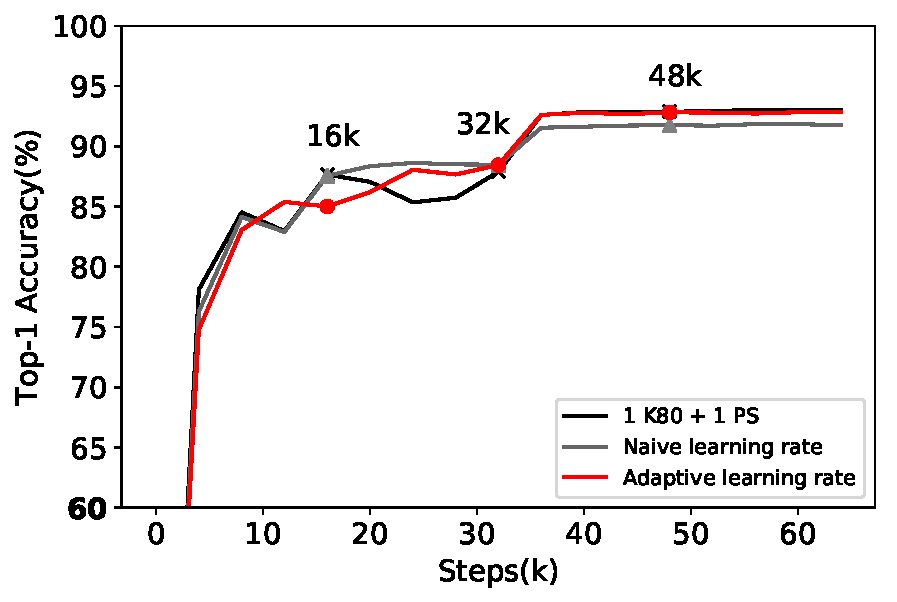
\includegraphics[width= 0.8 \columnwidth ]{adaptive_lr.pdf}
    \caption{\textbf{Benefits of dynamic transient distributed training and adaptive learning rate.}
    Dynamically scaling training cluster allows training to be finished 40.8\% faster compared to the static cluster. 
    By adaptively setting the learning rate based on the cluster size, we mitigate the accuracy degradation with naively using sparse mapping.}
%    Dynamically scaling training cluster allows training to be finished in 59.2\% of time compared to the static cluster. 
%    Naively using sparse mapping can lead to accuracy degradation. Adaptive learning rate based on the cluster size can mitigate the problem.}
    \label{fig:adaptive_lr}
\end{figure}
% 2.28 / 3.85 = 59.2%  100% - 59.2% = 40.8\%

Given the extended time it can take to train a model and the relative
volatility of transient server prices, it may make sense to dynamically add and
remove GPU servers during training. This would, for example, allow cloud
customers the flexibility to add cheaper transient servers to speed up
distributed training and ensure that they always have the best server
configuration given their budget and rapidly changing server prices. We refer
to this concept as \emph{dynamic transient clusters}.  

As existing distributed training frameworks do not natively support dynamic
clusters, we instead propose a technique called  \emph{sparse mapping} to
enabling dynamically adjusting training cluster configurations during runtime.
When using sparse mapping, cloud customers specify the maximum number of
workers (i.e. GPU servers), referred to as slots, allowed in the cluster. These
slots would then be filled \emph{opportunistically} during training.  For example, a
cloud customer can initialize a cluster with four slots and start training with one
initial GPU server; the other slots will be filled dynamically.  

%One challenge to implementing sparse mapping is  restricting the  network
%communication between the currently active workers and parameter servers. When
%the new workers join the cluster, the workers are presented with the same
%cluster configuration that already includes preallocated hostname and IP
%addresses. The new workers will then be able to communicate with the PS and
%start working on the training. 

% time (3.85 - 2.28) / 3.85  = 40.8%
% cost (3.11 -  2.44) / 3.11 = 21.5%
Intuitively, using sparse mapping allows cloud customers to  more efficiently
utilize transient servers depending on dynamic conditions, such as price. To
demonstrate this, we started a cluster  with a single \texttt{K80}. After every
16K steps, we added one additional \texttt{K80} server to the cluster. As shown
in Figure~\ref{fig:adaptive_lr}, the training finishes in 2.28 hours and is 40.8\% faster compared
to using a static cluster size.  Moreover, training with an elastic cluster
also leads to 21.5\% training cost savings when compared to training with the
static cluster size. However, we observe 1.17\% accuracy degradation for
training with a dynamic cluster size. This is because an important
hyperparameter, i.e., learning rate, that can affect training accuracy, is
currently calculated based on the number of workers supplied in the training
configuration, instead of the \emph{active} workers. We refer to the vanilla
way of leveraging sparse mapping without changing learning rate as \emph{naive
learning rate}. 

% 93.01 | 91.84 | 92.83  accuracy 

To further investigate the impact of incorrectly configured learning rate, we
implement an \emph{adaptive learning rate} that adjusts the learning rate based
the number of \emph{active} workers instead of the number of total workers
(slots). In Figure~\ref{fig:adaptive_lr}, we compare the achieved top-1 accuracy of training
with adaptive learning rate to both the baseline of training
with one \texttt{K80} server and training with a cluster with increasing number
of \texttt{K80} servers with naive learning rate. As shown, using adaptive learning rate can improve the
converged accuracy by 1\%. 

\textbf{Summary:} Sparse mapping provides a practical way to utilize transient
servers dynamically. However, naively utilizing sparse mapping can lead to
model accuracy degradation due to inappropriate learning rate. But adaptively scaling
learning rate to current number of workers can achieve 
%XX faster convergence and 
1\% higher accuracy compared to naive learning rate.

%%% 


\begin{figure}[t]
%
    \begin{subfigure}{0.24\textwidth}
    \centering
    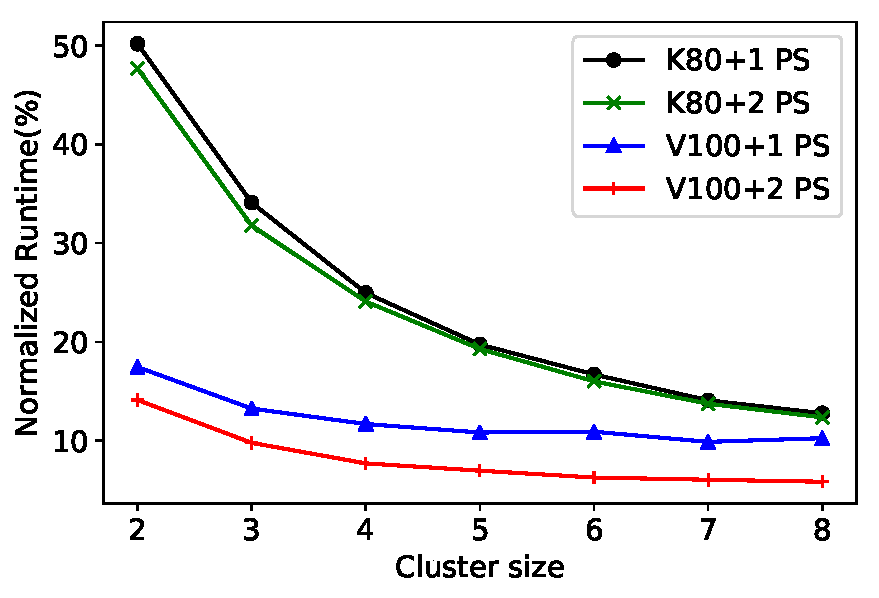
\includegraphics[width=\textwidth]{1ps_2ps_time.pdf}
        \caption{Training time.}
    \label{subfig:1ps2ps_time} 
    \end{subfigure}
\hfill
    \begin{subfigure}{0.24\textwidth}
    \centering
    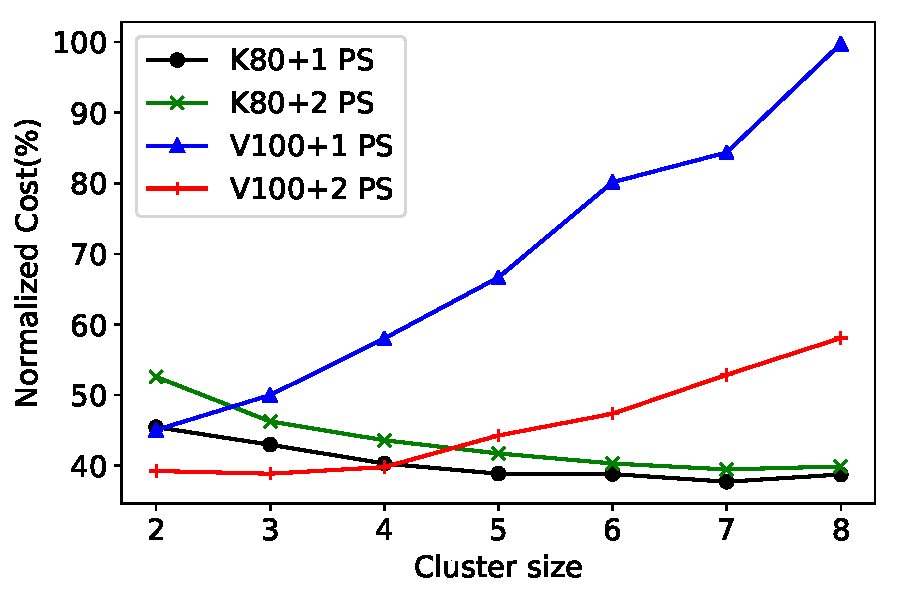
\includegraphics[width=\textwidth]{1ps_2ps_cost.pdf}
        \caption{Training cost.}
    \label{subfig:1ps2ps_cost} 
    \end{subfigure}
    %
    \caption{\textbf{Training performance bottleneck.} We measure the training time and monetary costs of scaling out with less powerful \texttt{K80} and more powerful \texttt{V100}, normalized to the single \texttt{K80} training. For \texttt{K80} clusters, the number of \texttt{PS} has little impact the training speed. In contrast, we observe up to 1.75X training speed using 2 \texttt{PS} in \texttt{V100} clusters compared to that of one \texttt{PS}. Consequently, the negligible speedup with using more expensive \texttt{V100} has lead to an almost linear increase of training cost. Note, training accuracy exhibits similar trend of decreasing with the cluster size as shown previously, and therefore we omit the accuracy comparison due to space limitation.
    % The cost of an additional PS is offset by the speedup of V100
    }
    \label{fig:1ps_2ps}
\end{figure}
% normalized time 10.26% to 5.85% = 1.75 at 8-V100



\begin{figure*}[t]
%
    \begin{subfigure}{0.32\textwidth}
    \centering
    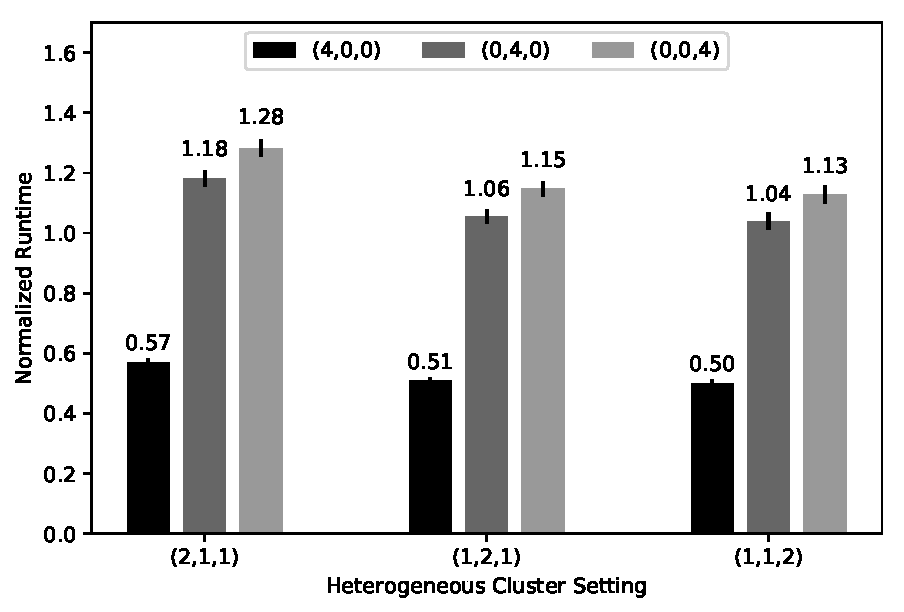
\includegraphics[width=\textwidth]{hetero_time.pdf}
        \caption{Training time.}
    \label{subfig:heter_time} 
    \end{subfigure}
\hfill
    \begin{subfigure}{0.32\textwidth}
    \centering
    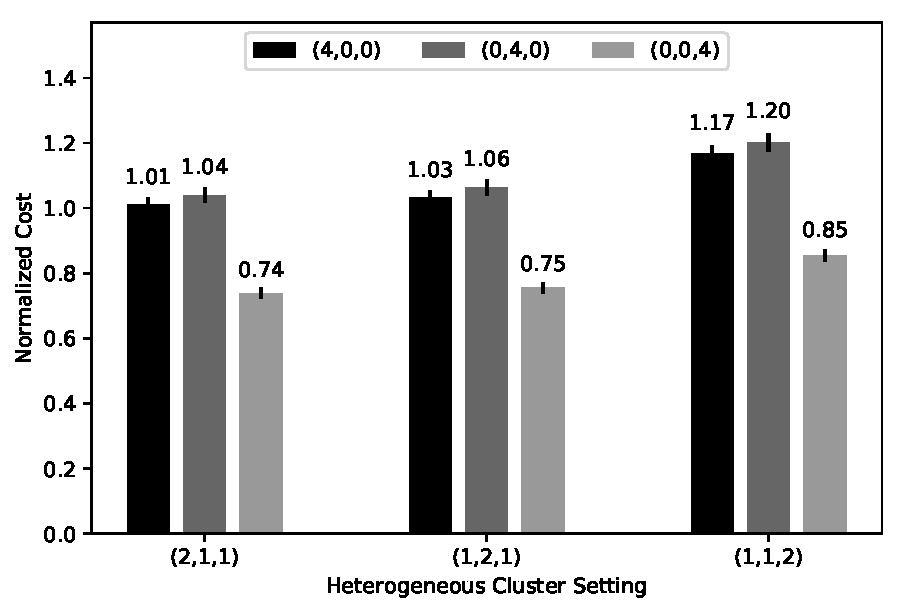
\includegraphics[width=\textwidth]{hetero_cost.pdf}
        \caption{Training cost.}
    \label{subfig:heter_cost} 
    \end{subfigure}
   %
   \hfill
    \begin{subfigure}{0.32\textwidth}
    \centering
    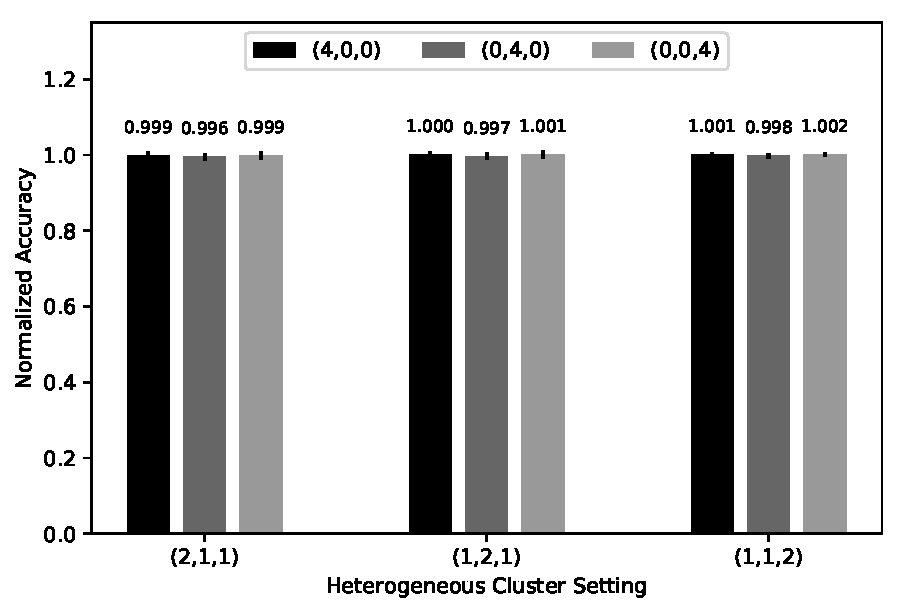
\includegraphics[width=\textwidth]{hetero_acc.pdf}
        \caption{Training accuracy.}
    \label{subfig:heter_acc} 
    \end{subfigure}
    %
    \caption{
%    \textbf{Training performance of heterogeneous clusters v.s. homogeneous clusters.}
    \textbf{Training performance with heterogeneous server sizes.}
    Mixing workers with less powerful GPU capacities can slow down the training by up to 28\% but lead to 26\% cost savings when compared to training with homogenous servers. However, there is no obvious accuracy drop.
     }
    \label{fig:heter_train}
\end{figure*}


\subsection{Implications of heterogeneous training}
\label{subsec:heter_train}


As empirically demonstrated previously, different classes of transient servers exhibit different
revocation probability, cost saving, and training speed trade-offs. This motivates the need to 
utilize a mix of GPU servers to balance such trade-offs in distributed training. We refer
to such clusters as \emph{heterogeneous} and in this section, we study two type of server heterogeneity---GPU types and server location.

%In some
%situations, it is desirable to utilize a mix of different server types to
%balance such trade-offs. We refer to such clusters as \emph{heterogeneous}. 
%  | 8 | V100+2PS | 95.86 | 5.85 | 58.08 |
% | 8 | V100+1PS | 95.69 | 10.26 | 99.77 |


We choose a cluster of \emph{four} servers for understanding the implications
of heterogenous training for two reasons. First, when scaling out with more powerful \texttt{V100}, we have observed 
that training time quickly plateaus after using more than four servers (Figure~\ref{subfig:1ps2ps_time}). That is, the training bottleneck has shifted from
the ability to parallelize the gradient computations to how fast the single \texttt{PS} can handle the weight pulling and gradient pushing from GPU servers. 
When using \emph{two} \texttt{PS} for \texttt{V100} clusters, we again observe training speed up for up to 1.75X compared to the single \texttt{PS} scenario. 
Second, under the current Google Compute Engine transient pricing models, when scaling out with more powerful \texttt{V100}, the monetary cost grows almost linearly, 
as shown in Figure~\ref{subfig:1ps2ps_cost}.

%because under the current transient pricing models,
%none of the distributed training configurations will exceed the training
%budget, and that PS starts to become the bottleneck, i.e., training with eight
%\texttt{V100} takes similar time compared to training with four \texttt{V100}
%servers. But if we launch the cluster of eight \texttt{V100} servers with two
%\texttt{PS} servers, we observe a significant speedup again. As shown in Figure~\ref{fig:1ps_2ps}


%

For understanding the first type of size heterogeneity, we conduct three baseline training scenarios of \emph{homogeneous} clusters that
consist of the same GPU server types, namely \texttt{K80}, \texttt{P100},
and \texttt{V100}. 
%
Let's define the training cluster with the number of GPU servers and types as
$(N_{K80}, N_{P100}, N_{V100})$, e.g., $N_{K80}$ denotes the number of \texttt{K80} used.  
In this experiment, we set the total number of GPU servers to be four, i.e., $N_{K80} + N_{P100} + N_{V100} = 4$. 
%
These homogeneous cluster configurations are represented as (4, 0, 0),  (0, 4, 0), and (0, 0, 4) respectively.
For each homogeneous cluster, we repeat the training ten
times and record the training performance. We construct three heterogeneous clusters with different mixes of all three GPU server types.
For example, we use the cluster configuration (2, 1, 1) to represent a cluster with two \texttt{K80} servers and one \texttt{P100} and one
\texttt{V100} each. To reiterate, one of intuitive use cases of heterogenous GPU types stems from simply unable to request for the desired transient servers.

In Figure~\ref{fig:heter_train}, we compare the training performance using heterogeneous clusters with that of homogenous clusters. When swapping out two(three) 
 \texttt{K80} for more powerful GPU servers, we observe up to 50\% speedup when compared to the homogeneous cluster of four-\texttt{K80} servers. 
 The heterogenous training  (1, 1, 2) with two \texttt{V100} incurs 17\% more monetary cost. Similarly, when swapping out two(three) \texttt{V100} for less powerful GPU servers, 
 we observe up to 28\% slowdown when compared to the homogeneous cluster of four-\texttt{V100} servers. The heterogenous training (2, 1, 1) with two \texttt{K80}  reduces the monetary cost by 26\%. Our evaluation suggests the benefits of mixing in more powerful transient GPU servers to significantly speedup the training with manageable cost increase and negligible accuracy impact. 
 
 
For understanding the second type of location heterogeneity, we compare the training performance of running distributed training within one single geographic region to across multiple regions. 
 We choose three US based regions, i.e., \emph{us-east1}, \emph{us-centra1} and \emph{us-west1} and represents the cross region cluster with number of servers running in the corresponding regions.  Note that \texttt{PS} is located in the data center with the largest number of workers. Similar to the need of using GPU servers of different capacities, the cost differences across regions are the key driven force for cross-region distributed training. As we can see from Figure~\ref{fig:cross_region_train}, splitting the GPU servers across different regions can lead to significant slowdown, up to 48\%. This is due to that GPU workers have to communicate with the \texttt{PS} through slower network connections. Even in the asynchronous training where workers do not need to wait for each other to receive the updated model parameters, the impacted workers contribute less towards completing the specified \emph{64K} steps, effectively slow down the overall training. Additionally, we do not observe obvious slow down when splitting the training in three regions, indicating that the network connections between two data center regions have similar performance. Interestingly, there is a slight increase in accuracy as the training slow downs. This suggests the potential opportunity to mitigate impact of cross-region trainings when transient costs are low enough. 


\textbf{Summary:} Training with heterogeneous GPU servers, either in terms of computation (size) or network (location) capacity, 
exhibits different tradeoffs in training cost and time. It is more intuitive to conduct distributed training with different GPU servers in the same data center, as the slow down is roughly proportional to the cost reduction. 
The saved money can be used to increase cluster size, therefore speedup both training and mitigate the revocation impacts. 
However, training across geographically dispersed data centers can incur signifiant training overhead, due to network communication. 
Our observations motivate the need to optimize the network communication of distributed training algorithm, in order to more effectively taking advantage of transient servers
with more dynamic supply.  


%\textbf{Summary:} We have observed ..... Mixing the use of different
%heterogeneous GPU servers only incur XX\% training speed degradation. Often the
%unit cost deduction can be up to YY\%, making it a worthy decision to speed up
%distributed training. Has/n’t on the converged accuracy ….  There are different
%types of heterogeneous that are specific to transient training that are worthy
%considering, e.g., utilizing servers in geographically dispersed data centers,
%Our observations motivate the need to re-architecture the current distributed
%training frameworks to more effectively taking advantage of transient servers
%with more dynamic supply.  



\begin{figure}[t]
%
    \begin{subfigure}{0.24\textwidth}
    \centering
    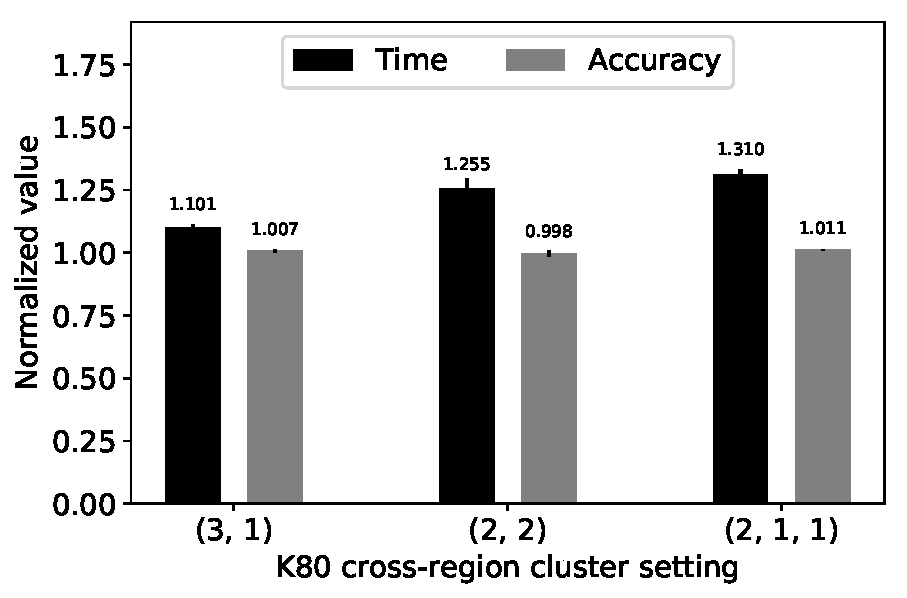
\includegraphics[width=\textwidth]{cross_region_k80.pdf}
        \caption{K80 clusters.}
    \label{subfig:heter_k80} 
    \end{subfigure}
\hfill
    \begin{subfigure}{0.24\textwidth}
    \centering
    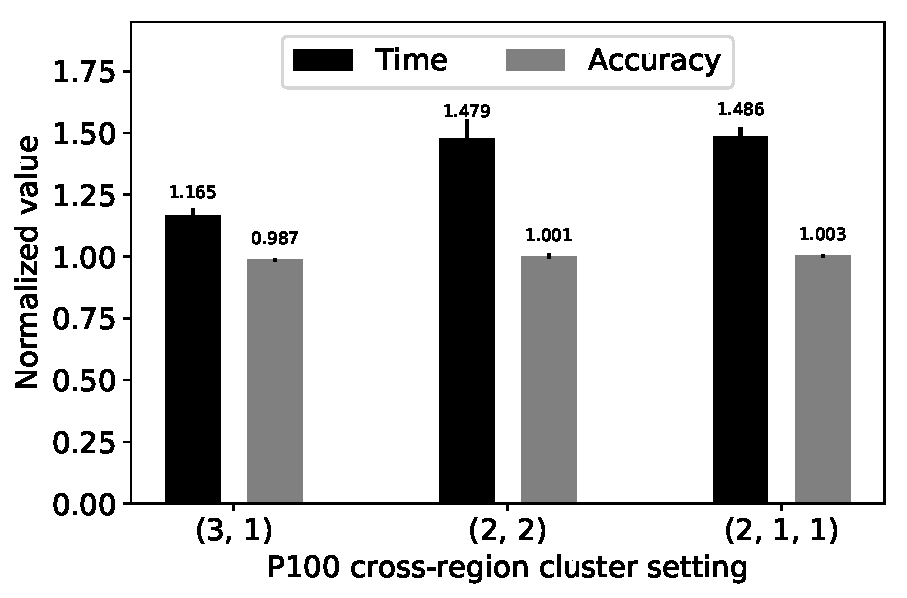
\includegraphics[width=\textwidth]{cross_region_p100.pdf}
        \caption{P100 clusters.}
    \label{subfig:heter_p100} 
    \end{subfigure}
    %
    \caption{\textbf{Training performance with heterogeneous server locations.}
    Distributed training using servers from different data center locations experience up to 48\% slow down when compared to training within the same region. 
    Interesting, splitting servers in three data centers show similar performance compared to two-regions based training.}  
%    \caption{\tian{placeholder}\textbf{Training performance of heterogeneous clusters v.s. homogeneous clusters.}
%    Mixing workers with less powerful GPU capacities can slow down the training by up to 28\% but lead to 26\% cost savings when compared to training with homogenous servers. However, there is no obvious accuracy drop.
%     }
    \label{fig:cross_region_train}
\end{figure}

%\begin{figure}[t]
%\centering
%    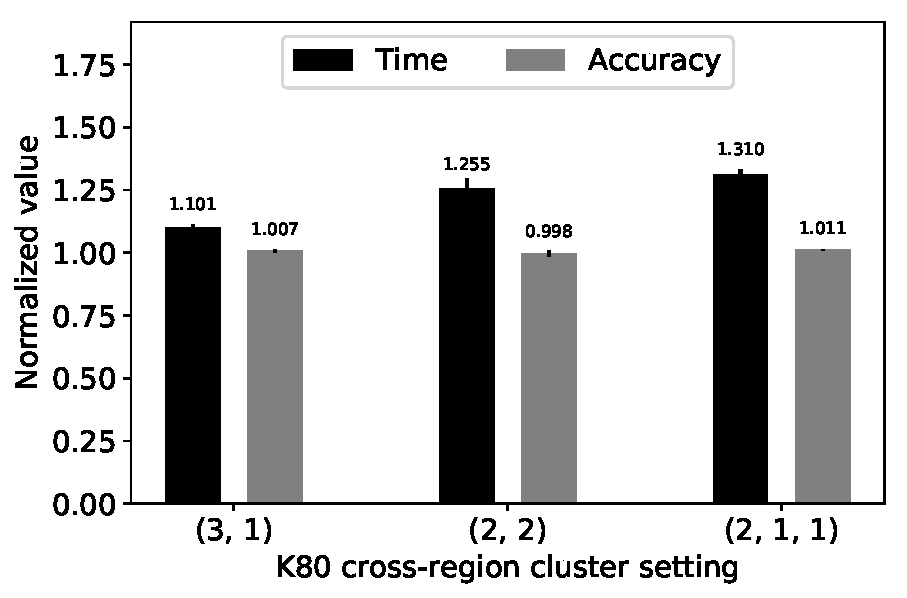
\includegraphics[width= 0.6 \columnwidth ]{cross_region_k80.pdf}
%    \caption{\textbf{Training performance with heterogeneous server locations.}
%    Distributed training using servers from different data center locations experience up to 48\% slow down when compared to training within the same region. 
%    Interesting, splitting servers in three data centers show similar performance compared to two-regions based training.}
%    Dynamically scaling training cluster allows training to be finished in 59.2\% of time compared to the static cluster. 
%    Naively using sparse mapping can lead to accuracy degradation. Adaptive learning rate based on the cluster size can mitigate the problem.}
%    \label{fig:cross_region_train}
%\end{figure}




